\section{Compound AI System Architecture}

PaperMemory is a compound AI system over a local PDF collection. The ingestion path renders PDFs into page artifacts and extracts selectable text where the PDF permits it. Each page can therefore carry an image, a caption or text snippet, a selectable-text manifest entry, and a quality label such as low-text or OCR-needed. This split matters because visual retrieval can still use page layout, while BM25 can use exact terms when text exists.

\begin{figure}[t]
  \centering
  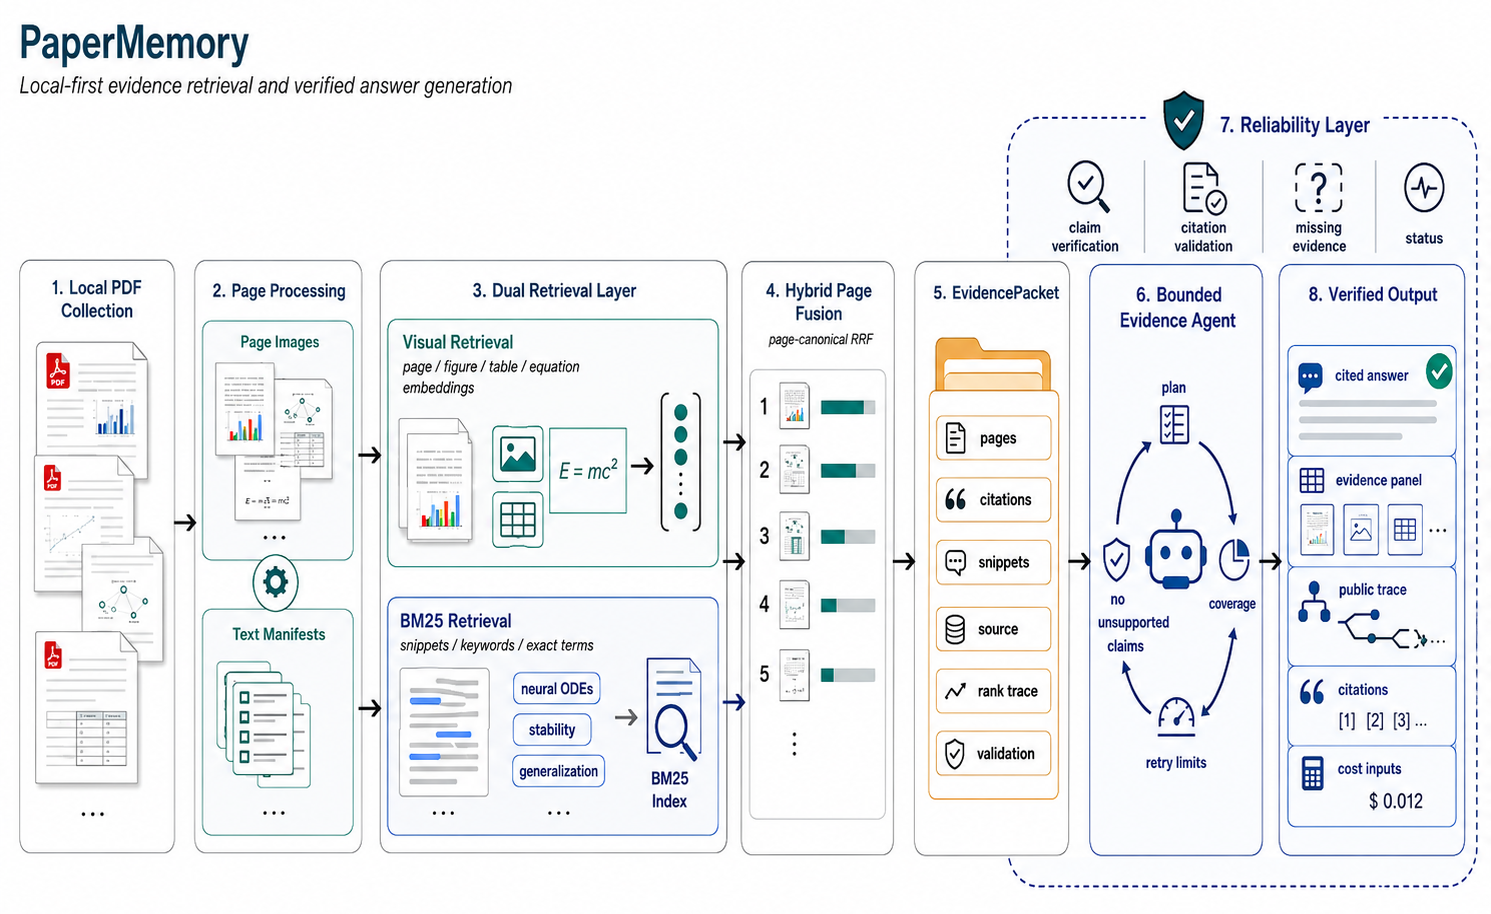
\includegraphics[width=\linewidth]{figures/papermemory_pipeline_figure1.png}
  \caption{PaperMemory pipeline with the reliability layer. The figure describes the report package over existing local artifacts; it does not add OCR, dense text retrieval, billing, or unrestricted agent actions.}
  \label{fig:pipeline}
\end{figure}


Retrieval has three implemented paths. The visual path retrieves page candidates from the page-image evidence surface. The BM25 path indexes the text manifests with $k_1=1.5$ and $b=0.75$. The hybrid path applies page-canonical reciprocal rank fusion with $k=60$, then collapses visual and text hits onto the same $(paper, page)$ unit. That canonical page key keeps the downstream citation grain stable even when the two retrievers disagree about score scale or rank source.

The EvidencePacket schema is the system boundary between retrieval and generation. A packet records the query, paper scope, accepted EvidenceUnits, accepted page citations, rank traces, source modality, validation state, and limits. The public packet excludes local filesystem paths and keeps stable evidence ids so that chat, trace logs, and report material can point back to the same page units \citep{paperMemoryEvidenceContract,paperMemoryChatPacket}. Generation is allowed to see packet context, but final citations are filtered back to accepted packet pages.

The reliability layer sits after packet construction and before the answer is treated as ready for the user. It plans evidence requirements from the question, checks whether the selected papers and claim types are covered, verifies answer claims against accepted evidence, and returns a visible \texttt{strong}, \texttt{partial}, or \texttt{insufficient} status. The status is a review signal, not a correctness certificate. It tells the user whether the packet supports the answer, where coverage is thin, and when the system should withhold or narrow a claim.

This architecture also connects to the product cost model. Reliability checks add planner and verification calls when enabled, while disabled reliability mode avoids that extra work. The cost stress test therefore belongs in the architecture story as a deployment control: stronger grounding can be purchased with more model work when the task warrants it, and lighter runs remain available for lower-risk exploration \citep{paperMemoryCostBenefit}.

\section{Agentic Autonomy and Implementation Logic}

PaperMemory's autonomy is bounded and server-verified. The agent does not browse freely, execute arbitrary tools, or attempt a complete literature review. It follows a small state machine over the selected paper scope. Planner output is treated as an untrusted hint, then the server clamps pass budgets, query counts, and final evidence size before retrieval or answer generation can proceed.

\begin{table}[t]
  \caption{Bounded agent trace states. The agent can retry for missing evidence, but server checks keep actions inside the selected paper scope.}
  \label{tab:agent-trace-summary}
  \centering
  \small
  \setlength{\tabcolsep}{3pt}
  \begin{tabularx}{\linewidth}{p{0.16\linewidth}YYYY}
    \toprule
    State & Agent action & Tool or component & Stop or transition & Safety boundary \\
    \midrule
    Rewrite & Prepare a scoped retrieval query from the user turn. & Server planner hint. & Move to first retrieval. & Planner output is validated and budget-clamped. \\
    Retrieve & Retrieve page evidence for the selected papers. & Hybrid, visual, or BM25 retrieval. & Build accepted EvidencePacket units. & Retrieval stays inside active paper scope. \\
    Analyze & Compare packet evidence with required claims. & Requirement planner and coverage check. & Stop as \texttt{sufficient} or request targeted retry. & Missing evidence is recorded as a limit. \\
    Retry & Search for uncovered requirements. & Coverage-gated retrieval retry. & Add only new accepted page units. & Pass count and query count are fixed by server limits. \\
    Check & Check whether retry changed the packet. & Evidence delta and dedupe check. & Stop as \texttt{no\_new\_evidence} when delta is zero. & Repeated retrieval cannot loop forever. \\
    Answer & Generate with final packet context and cite accepted pages. & Chat service and claim verifier. & Return answer plus reliability status. & Citations outside packet pages are stripped. \\
    \bottomrule
  \end{tabularx}
\end{table}


The implemented loop starts with query rewrite. The system prepares a conversation-aware retrieval query, then runs first retrieval through the selected retrieval mode, normally hybrid for scoped chat. Evidence analysis inspects the accepted packet units and records missing requirements. If coverage is incomplete and the budget remains, the orchestrator issues a targeted second retrieval rather than answering immediately. The retry is coverage-gated: it must seek missing evidence, deduplicate accepted units, and report whether the new pass changed the packet.

Stop reasons are explicit. A \texttt{sufficient} trace can answer after the first pass when the packet covers the question. A \texttt{no\_new\_evidence} trace stops after a retry produces no new accepted units. The answer step then uses the final packet, strips citations that do not match accepted pages, and attaches the reliability status from the requirement, coverage, and claim-verification checks. A \texttt{partial} answer can still be useful when it says which part is supported. An \texttt{insufficient} answer asks the user to revise scope or add evidence instead of filling the gap with unsupported prose.

The live controlled run exercises the same boundary. The successful image-context chat returned HTTP 200, six evidence rows, six citations, three included evidence images, and a final \texttt{sufficient} stop reason. The missing-evidence chat used a bounded second retrieval and ended with \texttt{no\_new\_evidence}, while the answer stated that the evidence packet did not support the requested mitochondrial ribosome profiling claim. The prompt-injection-style page stayed evidence rather than instruction: the answer treated the page text as untrusted and did not reveal keys, execute tools, or alter citations \citep{paperMemoryAgentTraces}.

\section{Baselines, Evaluation, and Technical Results}

The evaluation is a proof-of-capability package built from synthetic fixtures, deterministic regression tests, and a controlled local browser/API run. It is not a broad benchmark over scholarly PDFs. The synthetic retrieval suite has four papers, 12 pages, 12 golden questions, and three negative cases. The controlled local run used uploaded fixture PDFs and records UI flow, retrieval quality checks, bounded agent traces, and trust behavior. These artifacts support implementation claims, not claims about general corpus performance.

\begin{table}[t]
  \caption{Synthetic retrieval metrics from existing local artifacts. Higher is better for measured percentage columns.}
  \label{tab:retrieval-summary}
  \centering
  \small
  \setlength{\tabcolsep}{4pt}
  \begin{tabularx}{\linewidth}{YrrrrrY}
    \toprule
    Run & R@1 & R@3 & R@5 & Citation & Refusal & Boundary \\
    \midrule
    Keyword overlap baseline & 88.9\% & 100.0\% & 100.0\% & 100.0\% & 33.3\% & Same synthetic fixture; token overlap only, not LLM, BM25, VisRAG, or real corpus. \\
    Visual API baseline & 77.8\% & 100.0\% & 100.0\% & 100.0\% & 33.3\% & Synthetic smoke corpus; not a real PDF or real VisRAG result. \\
    BM25 text manifest & 88.9\% & 100.0\% & 100.0\% & 100.0\% & 100.0\% & Synthetic BM25-only text manifest fixture. \\
    Hybrid page fusion & 77.8\% & 100.0\% & 100.0\% & 100.0\% & 33.3\% & Synthetic page-canonical fusion; 27 units carry both traces. \\
    \bottomrule
  \end{tabularx}
\end{table}


The baseline comparison has one qualitative row and three measured retrieval rows. A GPT-only or manual narrative baseline has no Recall@k, citation-page correctness, or retrieval-level refusal score because it does not execute a page retriever or produce an EvidencePacket. The visual API baseline is the first measured synthetic row: Recall@1 is 77.8\%, Recall@3 and Recall@5 are 100.0\%, citation-page correctness is 100.0\%, and retrieval-level refusal correctness is 33.3\%. The BM25 text-manifest row improves Recall@1 to 88.9\% and refusal correctness to 100.0\% on the same synthetic setup, while preserving 100.0\% Recall@3, Recall@5, and citation-page correctness \citep{paperMemoryNode1,paperMemoryBm25Metrics}.

The hybrid page-fusion row should be read as provenance evidence. Its aggregate synthetic retrieval percentages match the visual baseline, but 27 returned units carry both visual and BM25 traces. That result confirms that page-canonical RRF can merge retriever evidence into a single packet unit without inventing a new citation grain \citep{paperMemoryHybridMetrics}. It does not show that hybrid retrieval is better on real paper collections.

The bounded evidence agent is evaluated through traces and regression behavior rather than Recall@k. The trace examples show accepted evidence ids, pass indexes, evidence deltas, stop reasons, and final packet limits. The controlled live run adds a more realistic smoke test: search and chat reached the local API, evidence cards appeared in the UI, citation chips were rendered, missing evidence stopped safely, and prompt-injection-style PDF text remained inside the evidence boundary. The main technical result is therefore narrower than a benchmark claim: the current implementation connects retrieval, EvidencePackets, bounded retries, reliability status, and UI evidence surfacing in a reproducible local workflow.
